\clearpage
\section{LW2 — Cinemática inversa algébrica}
\textbf{Fontes:} CSV de \source{lw2/}, capturas E.2 e \source{src/lite6\_ik/lite6\_ik/inverse\_kinematics.py}. O modelo direto usado é o da LW1, na convenção DH standard, mantendo a pose de \source{link\_eef} em \source{link\_base}.

\subsection{Parte A.1 — Derivação da solução fechada}
Seja $T_d=[R_d\ \mathbf p_d;\,0\ 1]$. A ponta está a $d_6=0{,}0615$ m do centro do punho ao longo de $\hat z_6$; logo,
\begin{equation}
\mathbf p_w=\mathbf p_d-d_6R_d\mathbf e_z=(x_w,y_w,z_w)^\top,\quad
h=z_w-d_1,\quad \rho=\sqrt{x_w^2+y_w^2}.
\end{equation}
Com $L_1=a_2=0{,}200$ m, $L_2=\sqrt{a_3^2+d_4^2}=\sqrt{0{,}087^2+0{,}2276^2}$ m e $\beta=\operatorname{atan2}(a_3,-d_4)$, há dois ramos para a base:
\begin{equation}
(q_1,r)=\bigl(\operatorname{atan2}(y_w,x_w),\rho\bigr)
\quad\text{ou}\quad
\bigl(\operatorname{atan2}(y_w,x_w)+\pi,-\rho\bigr).
\end{equation}
No plano ombro--cotovelo--punho, a lei dos cossenos dá
\begin{equation}
c=\frac{r^2+h^2-L_1^2-L_2^2}{2L_1L_2},\quad
\delta=\pm\arccos\bigl(\operatorname{clip}(c,-1,1)\bigr),\quad
q_3=\beta-\delta,
\end{equation}
\begin{equation}
q_2=\operatorname{atan2}(r,h)-\operatorname{atan2}\!\left(L_2\sin\delta,L_1+L_2\cos\delta\right).
\end{equation}
Assim cada ramo de $q_1$ admite até dois ramos do cotovelo. A orientação das três primeiras juntas, deduzida do produto DH da LW1, é
\begin{equation}
R_{03}=\begin{bmatrix}
c_1c_v&s_1&-c_1s_v\\s_1c_v&-c_1&-s_1s_v\\-s_v&0&-c_v
\end{bmatrix},\quad
v=q_2-q_3,\quad R_{36}=R_{03}^{\top}R_d,
\end{equation}
com $c_i=\cos q_i$, $s_i=\sin q_i$, $c_v=\cos v$ e $s_v=\sin v$. Para o punho regular, $s=\sqrt{R_{36,13}^2+R_{36,23}^2}>0$ e cada sinal $\sigma\in\{+s,-s\}$ fornece
\begin{equation}
q_4=\operatorname{atan2}\!\left(-R_{36,23}/\sigma,-R_{36,13}/\sigma\right),\quad
q_5=\operatorname{atan2}(\sigma,R_{36,33}),\quad
q_6=\operatorname{atan2}\!\left(-R_{36,32}/\sigma,R_{36,31}/\sigma\right).
\end{equation}
Cada ângulo é reduzido a $(-\pi,\pi]$; vetores equivalentes módulo $2\pi$ dentro de $\varepsilon_s=10^{-6}$ rad são devolvidos uma só vez. O algoritmo não usa iteração nem otimização.

\subsection{Partes A.2–A.4 — Ramos, alcance e singularidades}
Num caso regular há até $2\times2\times2=8$ soluções: inversão da direção da base, dois cotovelos e duas configurações do punho (sinal de $q_5$). O alvo é geometricamente inalcançável quando $c<-1$ ou $c>1$; o código tolera $10^{-12}$ além desses limites para não perder uma solução na fronteira por arredondamento. Na fronteira os ramos do cotovelo podem coincidir e a deduplicação remove repetições.

Quando os eixos das juntas 4 e 6 se alinham ($|\sin q_5|<\varepsilon_w=10^{-6}$), a pose não determina $q_4$ e $q_6$ separadamente. Para $q_5=0$, só a soma $q_4+q_6$ fica fixa módulo $2\pi$; a convenção é $q_4=0$ e $q_6=\operatorname{atan2}(R_{36,21},R_{36,11})$. O ramo de eixos opostos ($q_5=\pi$) tem relação angular análoga, mas está fora da gama permitida da junta 5. Se a projeção do centro do punho no plano da base for nula, o azimute requer cuidado geométrico adicional; os ensaios guardados não constituem uma campanha específica dessa singularidade.

\subsection{Seleção e nó ROS 2}
Para cada solução matemática $\mathbf q$, \source{select\_solution} substitui cada $q_i$ pelo equivalente $q_i+2\pi k$ dentro de \source{JOINT\_LIMITS} mais próximo do valor atual $q_{a,i}$. Descarta a solução se alguma junta não tiver equivalente admissível; das restantes escolhe $\arg\min\|\mathbf q-\mathbf q_a\|_2$. Sem solução executável, devolve \source{None}. O nó lê \source{/joint\_states} e \source{/lite6\_ik/target}, publica em \source{/lite6\_ik/solution} com a marca temporal do alvo ou regista \source{unreachable}/\source{out\_of\_range} sem publicar.

\subsection{Partes C e D — Verificação em Gazebo e no braço}
\begin{center}\scriptsize
\begin{tabular}{@{}lclrrrrrr@{}}\toprule
& & & \multicolumn{2}{c}{Gazebo vs. TF} & \multicolumn{2}{c}{Braço vs. TF} & \multicolumn{2}{c}{Braço vs. controlador}\\
Pose & Sim. & Real & mm & graus & mm & graus & mm & graus\\\midrule
A & atingida & atingida & 1,105 & 0,00155 & 1,188 & 0,03965 & 2,933 & 0,55723\\
B & atingida & atingida & 0,616 & 0,00120 & 0,585 & 0,02905 & 3,292 & 0,46126\\
C & atingida & atingida & 0,631 & 0,00117 & 0,651 & 0,02969 & 2,551 & 0,48339\\
D & atingida & atingida & 0,618 & 0,00106 & 0,523 & 0,03986 & 3,788 & 0,56863\\
U & recusada & recusada & — & — & — & — & — & —\\\midrule
Máximo A--D & & & 1,105 & 0,00155 & 1,188 & 0,03986 & 3,788 & 0,56863\\\bottomrule
\end{tabular}
\captionof{table}{Resultado por pose. A posição é em mm; o erro angular é o ângulo da rotação relativa.}
\end{center}
Em ambos os ambientes houve quatro poses atingidas, uma recusada (U, fora do alcance), zero rejeitadas. U foi recusada sem executar movimento para essa pose: P2.6 = 2/2. P2.4 (Gazebo vs. TF, $<2$ mm / $<0{,}05^\circ$) cumpre, incluindo os alvos $1{,}5$ mm / $0{,}01^\circ$. P2.5 é contra o controlador real, $<3$ mm / $<0{,}1^\circ$: $3{,}788$ mm / $0{,}56863^\circ$ \textbf{não cumpre}. A concordância com TF no braço não altera esta conclusão. Os dados não isolam se a discrepância vem de calibração, definição de TCP ou amostragem temporal. P2.2 e P2.3 são testes ocultos do docente; os estudos internos não os substituem.

\subsection{E.1 — Número de soluções}
\source{ik\_study count} produziu 500 linhas: 500/500 com oito soluções e com o vetor de origem encontrado. O erro interno máximo foi $6{,}14\times10^{-13}$ mm de posição e $2{,}58\times10^{-13}$ graus de orientação, contra a FK do próprio grupo.
\begin{center}\small
\begin{tabular}{@{}crrrrrrrr@{}}\toprule
N.º dentro das gamas & 1 & 2 & 3 & 4 & 5 & 6 & 7 & 8\\\midrule
N.º de poses & 4 & 171 & 14 & 212 & 1 & 3 & 8 & 87\\\bottomrule
\end{tabular}
\captionof{table}{Histograma E.1; o histograma do número total é: oito soluções em 500 poses.}
\end{center}
O gerador usa configurações regulares dentro das gamas, por isso os ramos da base, do cotovelo e do punho aparecem sem colapso nas 500 poses. Uma reavaliação das 4000 soluções com os limites do template encontrou 1576 violações da junta 3, 416 da junta 5, 328 da junta 2, e 12, 37 e 40 das juntas 1, 4 e 6, respetivamente; uma solução pode violar mais de uma gama. A restrição assimétrica da junta 3 é a principal redução do número executável. A contagem reproduziu \source{n\_in\_range} nas 500 linhas.

\subsection{E.2 — Todas as configurações para a pose A}
\source{ik\_check -p all:=true} registou oito soluções, quatro dentro das gamas e executadas (1, 2, 5, 6). As restantes foram rejeitadas sem movimento. Ângulos em graus, arredondados a uma casa:
\begin{center}\scriptsize
\begin{tabular}{@{}cll@{}}\toprule
N.º & $[q_1,q_2,q_3,q_4,q_5,q_6]$ & Resultado\\\midrule
1 & $[-28{,}1,31{,}0,106{,}1,-96{,}0,77{,}9,18{,}9]$ & atingida\\
2 & $[-28{,}1,31{,}0,106{,}1,84{,}0,-77{,}9,-161{,}1]$ & atingida\\
3 & $[-28{,}1,89{,}6,-148{,}0,-85{,}0,77{,}4,-29{,}6]$ & fora das gamas\\
4 & $[-28{,}1,89{,}6,-148{,}0,95{,}0,-77{,}4,150{,}4]$ & fora das gamas\\
5 & $[151{,}9,-89{,}6,106{,}1,102{,}1,83{,}9,-71{,}5]$ & atingida\\
6 & $[151{,}9,-89{,}6,106{,}1,-77{,}9,-83{,}9,108{,}5]$ & atingida\\
7 & $[151{,}9,-31{,}0,-148{,}0,93{,}7,77{,}0,-24{,}0]$ & fora das gamas\\
8 & $[151{,}9,-31{,}0,-148{,}0,-86{,}3,-77{,}0,156{,}0]$ & fora das gamas\\\bottomrule
\end{tabular}
\captionof{table}{Soluções de A: pares 1/2 e 5/6 invertem o punho; 1/2 vs. 5/6 trocam o ramo da base. Os ramos 3/4 e 7/8 têm $q_3=-148^\circ$, abaixo do limite inferior da junta 3.}
\end{center}
\begin{center}
\begin{tabular}{@{}cc@{}}
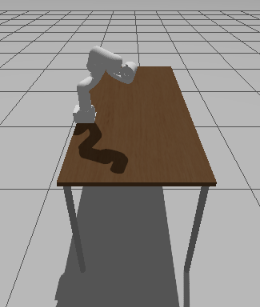
\includegraphics[width=0.39\linewidth,height=0.11\textheight,keepaspectratio]{images/E2_A_solucao_1.png} &
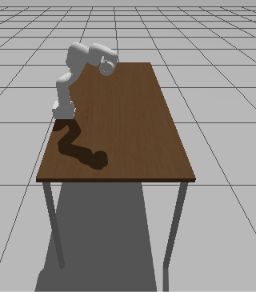
\includegraphics[width=0.39\linewidth,height=0.11\textheight,keepaspectratio]{images/E2_A_solucao_2.png}\\
Solução 1 & Solução 2\\
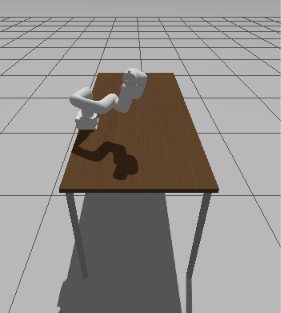
\includegraphics[width=0.39\linewidth,height=0.11\textheight,keepaspectratio]{images/E2_A_solucao_5.png} &
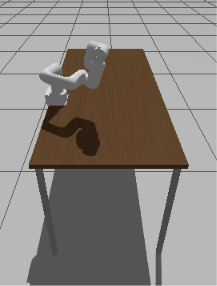
\includegraphics[width=0.39\linewidth,height=0.11\textheight,keepaspectratio]{images/E2_A_solucao_6.png}\\
Solução 5 & Solução 6
\end{tabular}
\captionof{figure}{Capturas do Gazebo fornecidas pelo grupo, uma por solução executada.}
\end{center}

\subsection{E.3 — Seleção a partir de S1–S4}
\begin{center}\small
\begin{tabular}{@{}clc@{}}\toprule
Arranque & Solução escolhida para A (graus) & Ramo E.2\\\midrule
S1 & $[-28{,}1,31{,}0,106{,}1,-96{,}0,77{,}9,18{,}9]$ & 1\\
S2 & $[-28{,}1,31{,}0,106{,}1,84{,}0,-77{,}9,-161{,}1]$ & 2\\
S3 & $[151{,}9,-89{,}6,106{,}1,102{,}1,83{,}9,-71{,}5]$ & 5\\
S4 & $[151{,}9,-89{,}6,106{,}1,-77{,}9,-83{,}9,108{,}5]$ & 6\\\bottomrule
\end{tabular}
\captionof{table}{Resultados dos quatro ficheiros \source{lw2\_ik\_sim\_A\_S1.csv} a \source{S4.csv}.}
\end{center}
Os quatro arranques colocam o braço perto de regiões diferentes do espaço articular. Depois do ajuste por $2\pi k$ e da exclusão dos ramos fora das gamas, a distância $\|\mathbf q-\mathbf q_{\mathrm{atual}}\|_2$ escolhe os ramos 1, 2, 5 e 6, respetivamente. A pose cartesiana final é a mesma; a proximidade articular muda.

\subsection{E.4 — Singularidade do punho}
\source{ik\_study wrist} registou 100 poses, sete soluções por pose (700 linhas). Em cada pose, uma das sete é a solução singular canónica com $q_4=0$ e $q_5=0$, conservando $q_4+q_6$ módulo $2\pi$. No primeiro caso, o vetor gerador tem $(q_4,q_6)=(-2{,}905177,0{,}944771)$ rad; a solução canónica devolve $(0,-1{,}960406)$ rad, a mesma soma. As outras seis soluções pertencem a outros ramos de base/cotovelo/punho e não precisam ter $q_5=0$. O erro interno máximo foi $9{,}92\times10^{-12}$ mm e $9{,}19\times10^{-12}$ graus, contra a FK do próprio grupo.

\textbf{Vídeo.} \href{\repo/lw2/lw2_ik_real.mp4}{Execução da LW2 no braço}: o verificador visita S0, executa A–D e regista U como recusada, sem comandar a pose fora do alcance. O ficheiro tem 66,32 s.
